\chapter{Introdução}\label{chp:intro}

\section{Apresentação}\label{sec:presentation}
O conceito de \textit{smart houses} (casas inteligentes) tem ganhado grande destaque no meio acadêmico e no mercado nos últimos anos, com o desenvolvimento de tecnologias interativas e de redes sem fio \cite{harper2006}. É intuitivo que a possibilidade de concretização desse conceito de casa inteligente, viabilizado pelo avanço de tais tecnologias, foram decisivos  para a sua popularização. Não surpreende, pois, que em 2016, a empresa de consultoria Gartner tenha destacado o item ``casa conectada'' em seu relatório anual de tendências de tecnologias emergentes, denominada \textit{Hype Cycle}, como pode ser visto na Figura \ref{fig:gartner}.

\begin{figure}[h]
	\centering
	\caption{Relatório \textit{Hype Cycle} da Gartner destacando a tecnologia de casas conectadas.}
  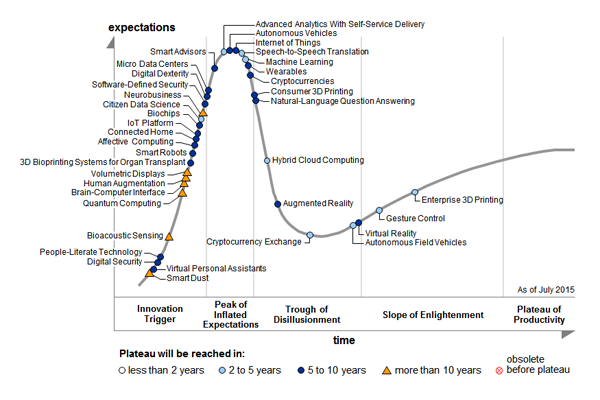
\includegraphics[width=0.9\textwidth]{imagens/gartner.png}
  \label{fig:gartner}
  
  Fonte: \cite{gartner}
\end{figure}

O conceito de casa inteligente é definido por \cite{jiang2004} como ``uma residência incorporando uma rede de comunicações que conecta serviços e equipamentos elétricos, permitindo que eles sejam controlados remotamente, monitorados ou acessados''. Esta definição explicita o caráter interativo e automatizado inerente ao conceito, abrindo uma margem muito grande de possíveis aplicações de utilidade social. Dentre tais aplicações, inclui-se prover automação residencial e conectividade social \cite{harper2006}, além de fornecer um ambiente seguro e monitorável a idosos ou deficientes \cite{chan2008}.


\section{Soluções existentes}\label{sec:solutions}
Acompanhando a popularização do conceito de \textit{smart houses}, diversas soluções e plataformas foram desenvolvidas e lançadas no mercado. Como exemplos, pode-se citar o Apple HomeKit \cite{homekit}, Wireless Sensor Tags \cite{wsensortags}, WigWag \cite{wigwag} e o Samsung SmartThings \cite{smartthings}.

Todas as soluções citadas, à exceção do Apple HomeKit, seguem uma arquitetura similar. Os sensores e atuadores distribuídos pela residência são conectados a um controlador central, responsável por coletar leituras dos sensores e comandar ações aos atuadores. Além disso, este controlador se conecta a um servidor em nuvem, que centraliza o armazenamento de dados e fornece uma interface aos usuários para monitorar e definir o estado da residência.

A solução desenvolvida pela Apple baseia-se na utilização dos dispositivos móveis da empresa para efetuar o monitoramento e controle mencionados. Assim, ela é fortemente dependente do ecossistema Apple para o funcionamento, especialmente pelo fato de o suporte ser dado somente pelo sistema operacional proprietário iOS. No entanto, a empresa permite o desenvolvimento de dispositivos de terceiros compatíveis com o HomeKit, através da disponibilização de um \textit{framework} próprio. Os produtos desenvolvidos devem ser certificados pela Apple, processo este envolvendo a obtenção de licenças e submissão a análises.

O Wireless Sensor Tags apresenta uma solução baseada em um controlador local (\textit{tag manager}) conectado à Internet, disponibilizando diversos sensores compatíveis com o controlador. Basicamente, ele permite a utilização de um aplicativo para monitorar os sensores, definindo alertas de acordo com as leituras obtidas. Não é mencionado suporte a atuadores, nem a possibilidade de desenvolver dispositivos de terceiros compatíveis com o sistema.

O WigWag também é uma solução baseada em um controlador local (aqui denominado \textit{relay}), podendo operar conectado à nuvem ou não. A interface disponível possibilita a definição de regras de automação, controlando atuadores caso determinadas leituras de sensores forem verificadas. O aspecto mais interessante desta solução é a capacidade de integrar dispositivos de terceiros utilizando uma plataforma que se auto-denomina de código  aberto, chamada deviceJS. No entanto, o acesso a esta plataforma se encontra fechado no momento de escrita deste relatório.

Por fim, de modo análogo às demais, a solução SmartThings baseia-se em um controlador local (\textit{hub}), que se conecta a servidores em nuvem próprios da Samsung. Esta solução destaca-se pelo foco dado à integração com dispositivos de terceiros, possuindo a documentação mais completa dentre os exemplos analisados. Tal integração baseia-se em dois componentes de software básicos: \textit{device handlers} e \textit{smart apps}. Os \textit{device handlers} funcionam como \textit{drivers}, sendo executados no controlador local. A função deles é traduzir comandos de alto nível do controlador (e.g., ligar a luz) para sinais de controle específicos do dispositivo. Os \textit{smart apps}, por sua vez, adicionam a parte de inteligência do sistema, permitindo a criação de regras de automação de modo similar ao WigWag. A empresa disponibiliza aos desenvolvedores um ambiente de desenvolvimento completo para implementar os componentes citados.

\section{Motivação e Objetivos}\label{sec:goals}
Conforme mencionado, o conceito de \textit{smart houses} tem o potencial de trazer vários benefícios aos usuários. Logo, é interessante incentivar o desenvolvimento de sistemas abertos, desvinculando-os de empresas e serviços específicos e tornando-os mais flexíveis para o usuário. Note que, das soluções apresentadas, nenhuma é genuinamente aberta. As soluções WigWag e Samsung SmartThings são as que mais se aproximam dessa ideologia ao disponibilizar plataformas em código aberto para integrar dispositivos de terceiros, mas ainda possuem protocolos de comunicação proprietários (ao menos não documentados) que são dependentes de controladores e servidores em nuvem proprietários.

O grupo acredita que a existência de um protocolo de comunicação que possibilite a troca de dados e a coordenação dos dispositivos da rede de sensores resulte em maior flexibilidade aos desenvolvedores desses equipamentos. Isso ocorre pois existiria uma garantia de que um dispositivo aderente ao protocolo funcione com quaisquer outros dispositivos ou controladores que também o respeitem, removendo quaisquer dependências com soluções ou fabricantes existentes.

Além disso, a inteligência contida nas \textit{smart houses} é razoavelmente limitada nas soluções existentes. Conforme apresentado anteriormente, toda a inteligência é provida pelo usuário, que configura manualmente regras envolvendo sensores e atuadores. Ou seja, uma casa que se autoconfigurasse ou sugerisse regras ou ações ao usuário teria destaque no mercado, eliminando ainda mais a intervenção do usuário e fornecendo assim uma  experiência altamente customizada.

Um último aspecto a se mencionar é o fato de nenhuma das soluções estar disponível no mercado brasileiro no momento de escrita deste relatório (início de 2016). Os equipamentos do SmartThings, por exemplo, nem sequer são enviados ao Brasil, estando, pois, indisponíveis para importação. Vê-se a necessidade, portanto, do desenvolvimento de uma solução nacional para o segmento das \textit{smart houses}.

Assim, pode-se dividir o objetivo do presente projeto nos seguintes itens:
\begin{enumerate}[\quad (i)]
	\item Projetar e implementar uma plataforma aberta que possa ser utilizada como base para a construção de uma solução local de automação residencial, e
	\item Projetar e implementar uma metodologia envolvendo aprendizagem de máquina que permita geração de regras de automação baseadas no comportamento do usuário.
\end{enumerate}

Cabe ressaltar desde já que este trabalho não será focado nos aspectos de segurança do protocolo, como detalham as seções de não-escopo deste documento. O foco dado é em prover as funcionalidades básicas de uma rede de sensores e atuadores doméstica, permitindo a interoperabilidade entre os dispositivos.

\section{Organização do Documento}
O documento está organizado da seguinte forma. O capítulo \ref{chp:espec_metodologia} contém a especificação de requisitos, os não-escopos e a metodologia adotada no projeto; o capítulo \ref{chp:redesensores} trata do desenvolvimento do protocolo a ser executado na rede local de dispositivos, contemplando o objetivo (i); o capítulo \ref{chp:serviconuvem} aborda serviços em nuvem e o aplicativo móvel de interface com o usuário, incluindo-se o algoritmo de aprendizagem proposto no objetivo (ii); o capítulo \ref{chp:testes} descreve o procedimento de teste modular e de integração adotado no projeto, e o capítulo \ref{chp:conclusoes} contém uma análise crítica do grupo em relação aos resultados e ao preocesso de desenvolvimento deste projeto.